\title{Analysis of CWRU Student Course Evaluations}
\author{
        Benjamin Kaplan and Stephen Johnson\\
}
\date{\today}

\documentclass[12pt]{article}
\usepackage{fullpage}
\usepackage{url}
\usepackage{graphicx}
\usepackage{wrapfig}
\usepackage{subfigure}
\usepackage{amssymb}

\begin{document}
\maketitle

\section{Introduction}
Every semester, students at Case are asked to evaluate their classes. This provides a huge wealth of information but it is fairly useless it its raw form. Using the data collected for each class, we can find out more about how students feel about academics at Case Western Reserve. For our analysis, we are utilizing all course evaluations submitted for undergraduate courses at Case Western from the fall of 1997 through the fall of 2006. Although the surveys are voluntary, subjecting them to selection bias, they have a high response rate. We used a custom script (written in Python) to parse the data. The source code used to generate the graphs can be seen at \url{http://www.github.com/irskep/cwru-courses}.

\section{Hypotheses}
We decided to test the popular belief among students that the engineering classes here are more difficult and have a higher workload than the courses offered for the arts and sciences majors. In addition, we believed that SAGES classes would be significantly less popular than all the other courses.

In addition to comparing the different sets of classes, we thought that as the average class standing of the students increased, the course score would increase as well since more of the upper level classes are electives or are part of the student's chosen major while classes consisting mostly of freshmen and sophomores would be more general education classes.

Finally, we plan on looking at changes in student behavior over the 10 year time period. We believed that the ratings would improve slightly over the time period. Some of the questions asked on the survey, such as whether the class encourages critical thinking, identifies a major focus of universities in recent years.

\section{Methodology}
To start our analysis, we had to take our parsed data and clean it up. In our initial parsing, we found several missing pieces of data. In particular, the data for ENGR 145 and CHEM 111 (the introduction to chemistry classes for engineers) left values blank in the data file. Also, there were some typos. A few times, the course code had the letter ``O'' instead of the number 0.

Finally, we had to filter out irrelevant data. The first thing we did on reading in the data was to filter out graduate courses, which have a course number greater than 400. In addition, we had to filter out classes that had no responses for a particular category, such as rating the TA in courses that didn't have a TA. 

\section{Course Rating and Academic Standing}
To test our hypothesis that courses with more advanced students would get higher ratings, we mad a scatter plot of course ratings over academic standings and fit a regression line to it. The standard error on the line was very high, about 0.7 in a range of 0.0-4.0, so it is clear that a student's standing has little effect on course ratings. Our hypothesis was disproven.

\begin{center}
    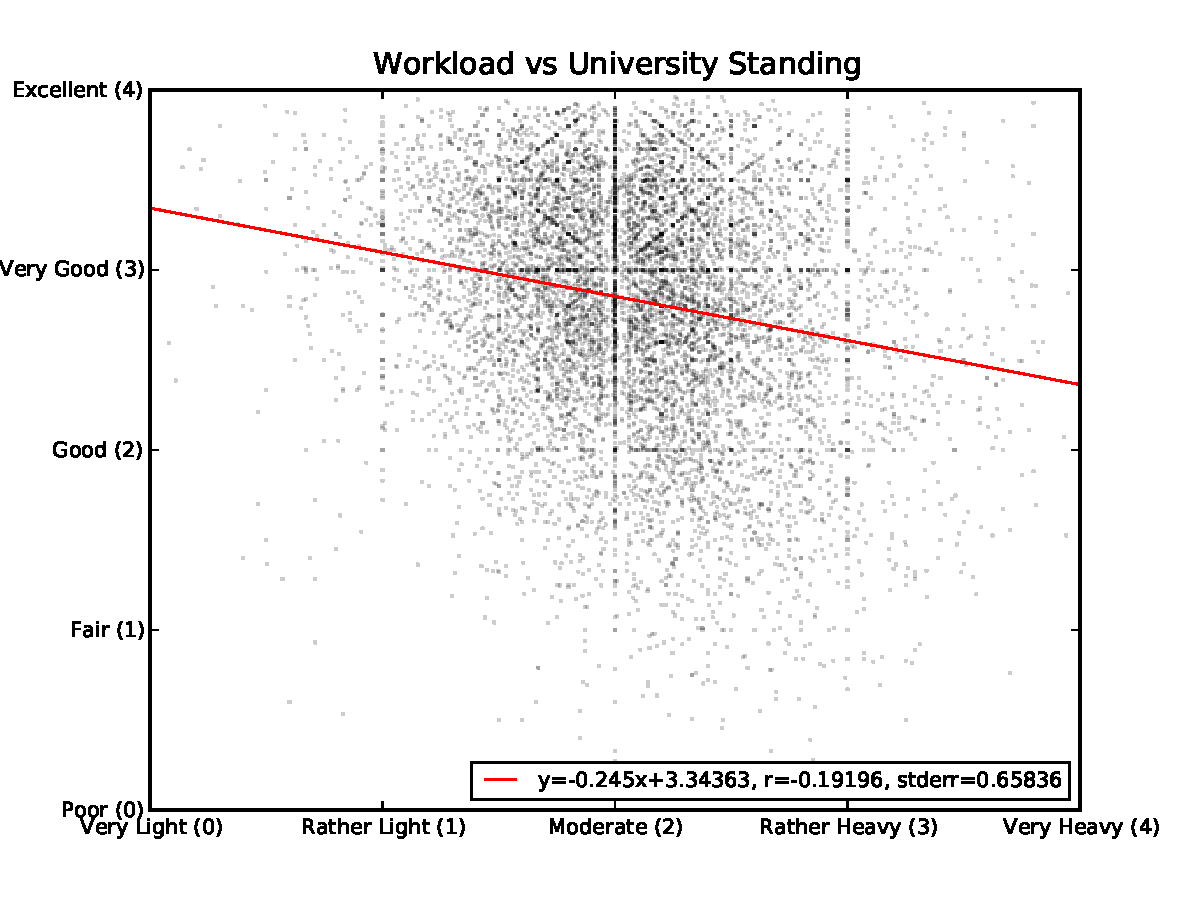
\includegraphics[width=5in]{figures/rating_vs_standing.pdf}
\end{center}

\section{Arts and Sciences vs. Engineering}
We observed several things with this wealth of data (we had over 8,000 data points). First of all, we know, with a confidence level of 99.9\%, that classes for the college of arts and sciences rate higher than classes for the school of engineering. Using the scale where 0 = poor and 4 = Excellent with the other variables in between, the 1,595 classes in the School of Engineering received an average rating of 2.56, with a standard deviation of .63398. The 6,510 classes in the College of Arts and Sciences had an average rating of 2.92 with a standard deviation of 0.65572. Using a 2-sample Student's T distribution gave a T score of about -20, which corresponds to a probability of less than .000001.

In addition, an analysis of course difficulty shows that students consider engineering classes to be harder than Arts and Sciences classes. The engineering classes had an average difficulty score of 2.28 $\pm$ 0.54851 while the arts and sciences classes had an average difficulty of 2.05123 $\pm$ 0.52131.

We also ran a T-test based on the students' ratings of the course TA. In this case, the Arts and Sciences rated significantly higher than Engineering. The College of Arts and Sciences rated their TAs 2.8 while the School of Engineering TAs had an average rating of 2.33. The 2-sample T-Test yielded a T value of -14.95. It's interesting to note, however, that a much higher percentage of the engineering classes rated the TAs (1345 out of 1595) than the Arts and Sciences classes (3108 out of 6510).

\section{SAGES}
We also examined the early data from the SAGES program. The 466 SAGES classes in the dataset had an average course ranking of 2.380 $\pm$ 0.804. The other classes 8968 classes had an average ranking of 2.855 $\pm$ 0.655. This yields a T score of -15.09, suggesting that there is an extremely high probability that Sages classes rank lower than non-SAGES classes.

However, the difference in workload between SAGES classes (2.12244$\pm$0.4) and non-SAGES classes (2.088$\pm$0.531) was not significant. Based on this early data, students were not pleased with the SAGES program even though the courses themselves weren't more time consuming than their other classes.

\section{Trends Across Time}
In addition to comparing the different groups of courses, we also searched for trends across time. Our data covers 19 semesters, from the fall of 1997 to the fall of 2006. We plotted the average score in several categories, stratified again by school. The graphs containing the data and regression lines for the College of Arts and Sciences, the School Engineering, and SAGES are included in Appendix B, labeled with the question numbers from the survey. The Weatherhead School of Management and the Mandel Center were excluded due to an insufficient number of data points.

Overall, we noticed that there was very little change during the 10 year period observed. Even though some of the regression lines were statistically significant ($> 95\%$), the slope of the line was minute. One trend we noticed is that the SAGES results are very scattered. The results for SAGES vary greatly from year to year. The SAGES results also had high standard errors for each semester (marked on the charts). This is probably because SAGES was still in its experimental stages at the time and the seminar format means that the students' experiences will depend on the professor and the subject of the seminar.

The individual regression lines for the College of Arts and Science and the School of Engineering confirm our analysis of the overall ratings, i.e. that engineering classes are rated lower and more difficult.

The only major feature evident from the graphs is that the ratings are slowly rising in all categories except for course pace and workload, which have been declining since the start of our data. However, all lines are very flat, with the exception of SAGES as mentioned above. In general, courses in 2006 were slightly easier for students than in 1997, or at least students perceive them that way.

Given the above observation, we decided to correlate course ranking and workload with the hypothesis that easier courses get rated higher by students. The resulting scatter plot and regression line is below. As you can see, it has a high $r$ value, but there is a distinctive downward slope in ranking as the workload becomes heavier.

\begin{center}
    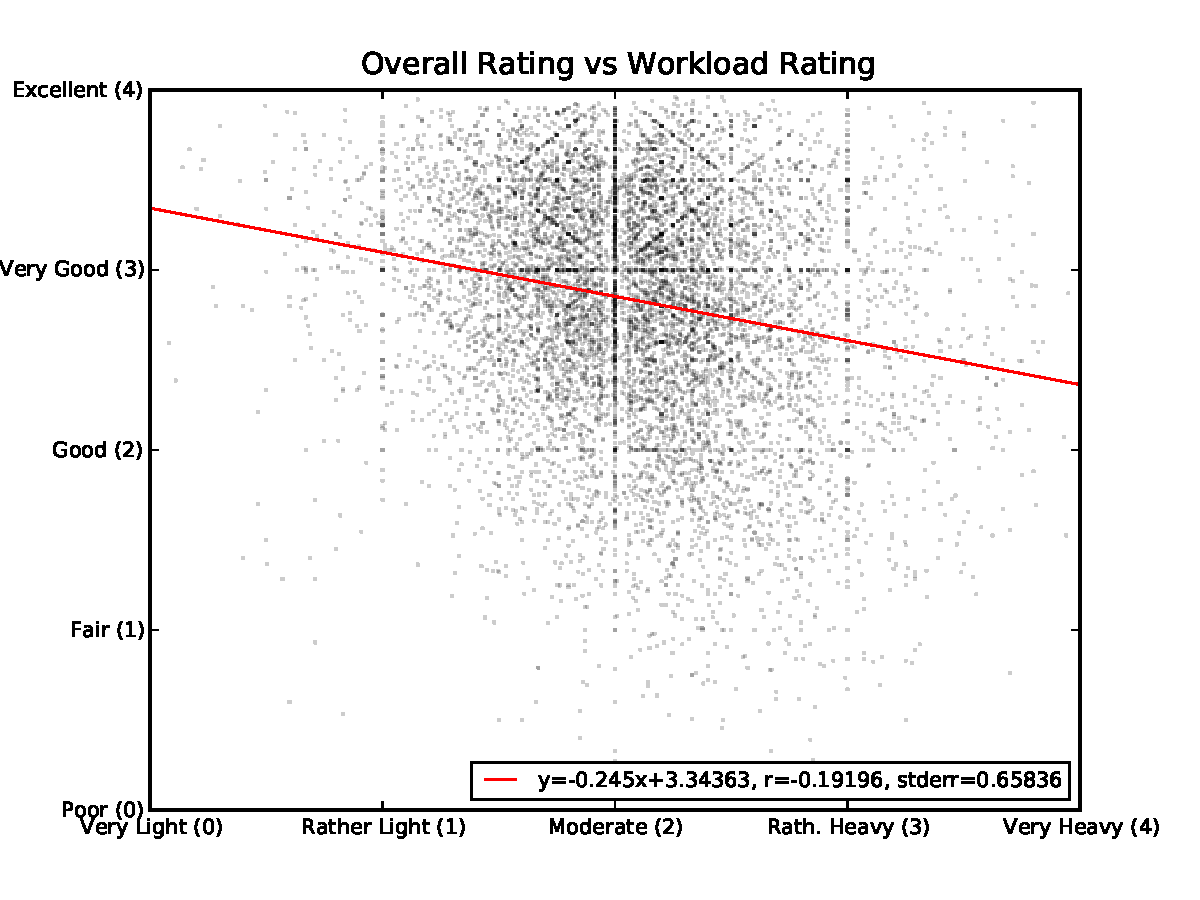
\includegraphics[width=5in]{figures/rating_vs_workload.pdf}
\end{center}

\section{Conclusions}
Our most reliable conclusion is that courses offered by the College of Arts and Sciences are rated better in every category that students consider positive. This conclusion is shown to be true over all points of time by the graphs included in Appendix B.

Our hypotheses about SAGES were neither confirmed nor disproven due to the relatively small and inconsistent data set. More data is needed to form an accurate conclusion.

Our hypothesis about a student's standing as a freshman, sophomore, junior, or senior was disproven by the high $p$ value of the scatter plot.

\appendix

\section{Course Evaluation Questions}
\begin{verbatim}
 1. HOW DOES THIS COURSE FIT INTO YOUR ACADEMIC PROGRAM
 2. WHAT IS YOUR CURRENT STANDING IN THE UNIVERSITY
 3. RATE THE PACE OF THE COURSE 
 4. RATE THE WORK LOAD OF THE COURSE
 
 Rated SA/A/M/D/SD/NA:
 5. INSTRUCTOR HAS AN EFFECTIVE COMMAND
 6. INSTRUCTOR SPEAKS AND WRITES CLEARLY
 7. EXPECTATIONS OF INSTRUCTOR ARE CLEAR
 8. COURSE PROCEDURES CLEARLY EXPLAINED
 9. ABLE TO MOTIVATE STUDENTS
10. ENCOURAGING QUESTIONS AND DISCUSSIONS
11. COURSE STIMULATES CRITICAL THINKING
12. PROPER LEARNING ATMOSPHERE PROVIDED
13. STUDENTS ARE INFORMED OF THEIR PROGRESS
14. GRADING IS DONE FAIRLY
15. ADEQUATE ASSISTANCE IS AVAILABLE
16. TEXTBOOK/CLASS MATERIAL ARE USEFUL

 Rated E/VG/G/F/P/NA
17. THE COURSE
18. THE INSTRUCTOR
19. THE TEACHING ASSISTANT (IF APPLICABLE)
20. THE LABORATORY (IF APPLICABLE)
\end{verbatim}

\section{Graphs}
\begin{center}
    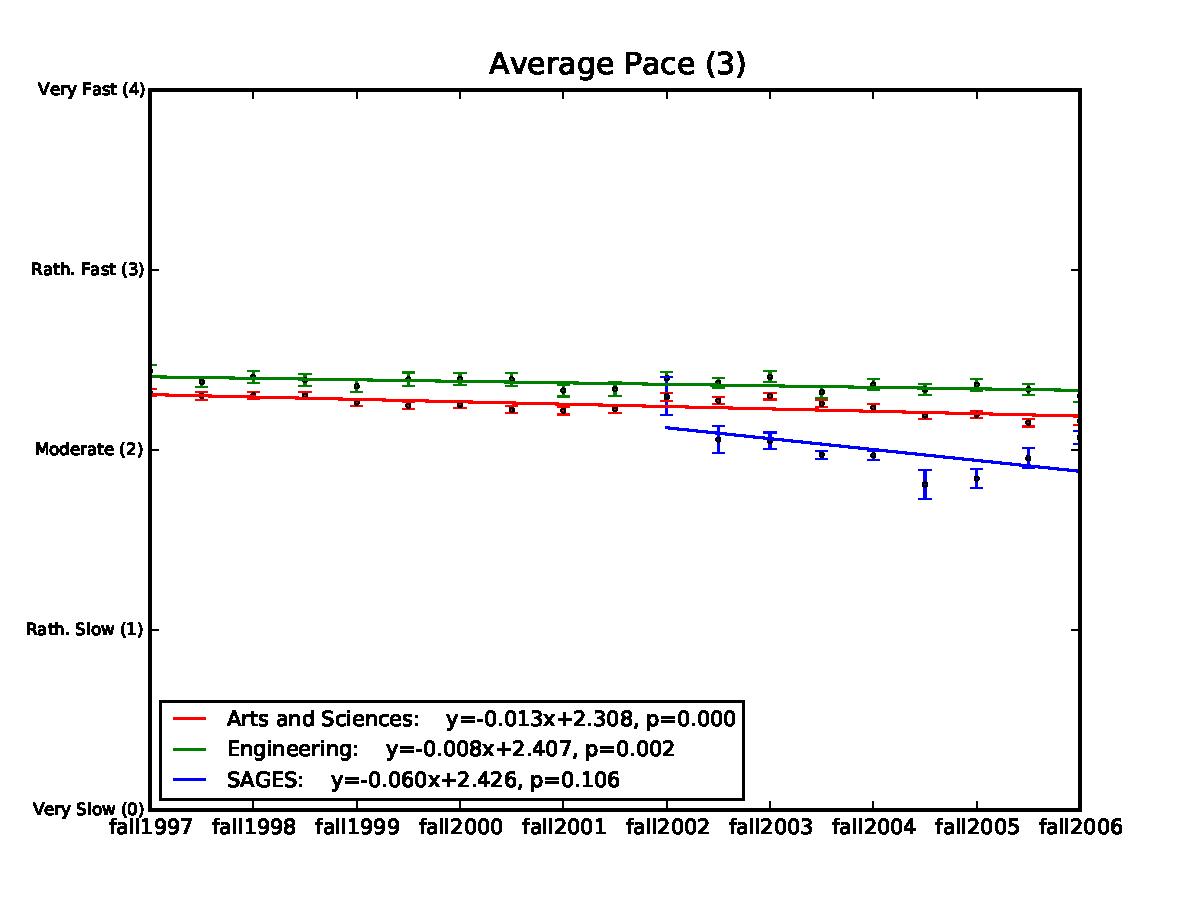
\includegraphics[width=5in]{figures/3_pace_over_time.pdf} \\
    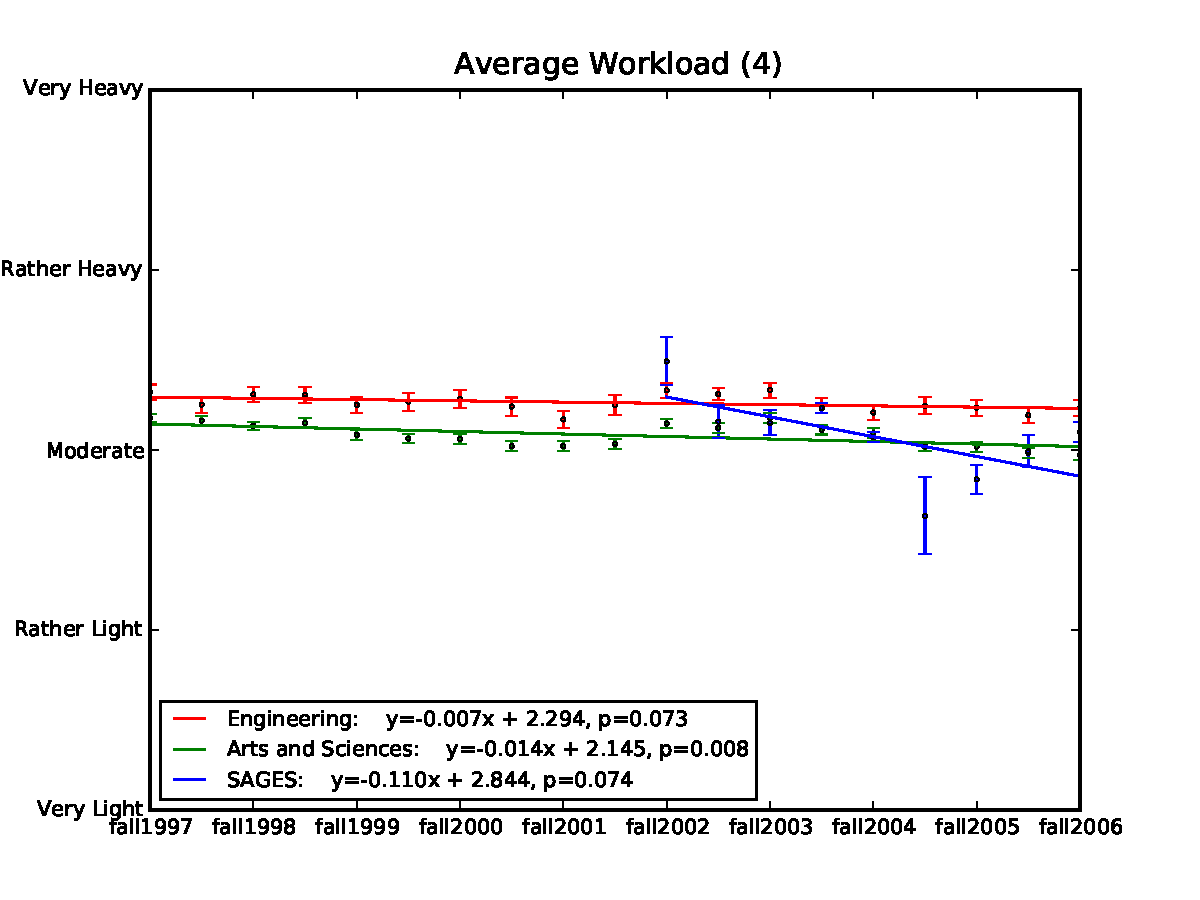
\includegraphics[width=5in]{figures/4_workload_over_time.pdf} \\
    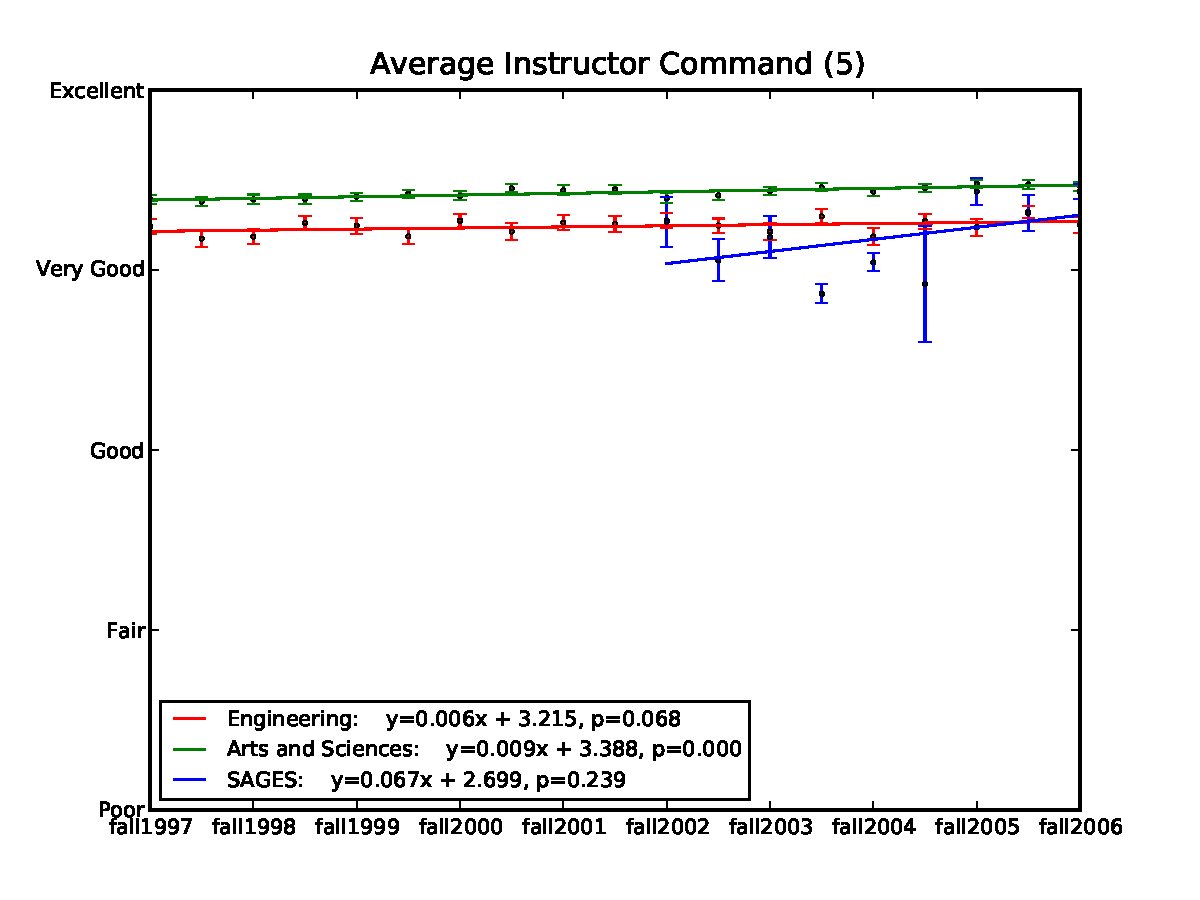
\includegraphics[width=5in]{figures/5_command_over_time.pdf} \\
    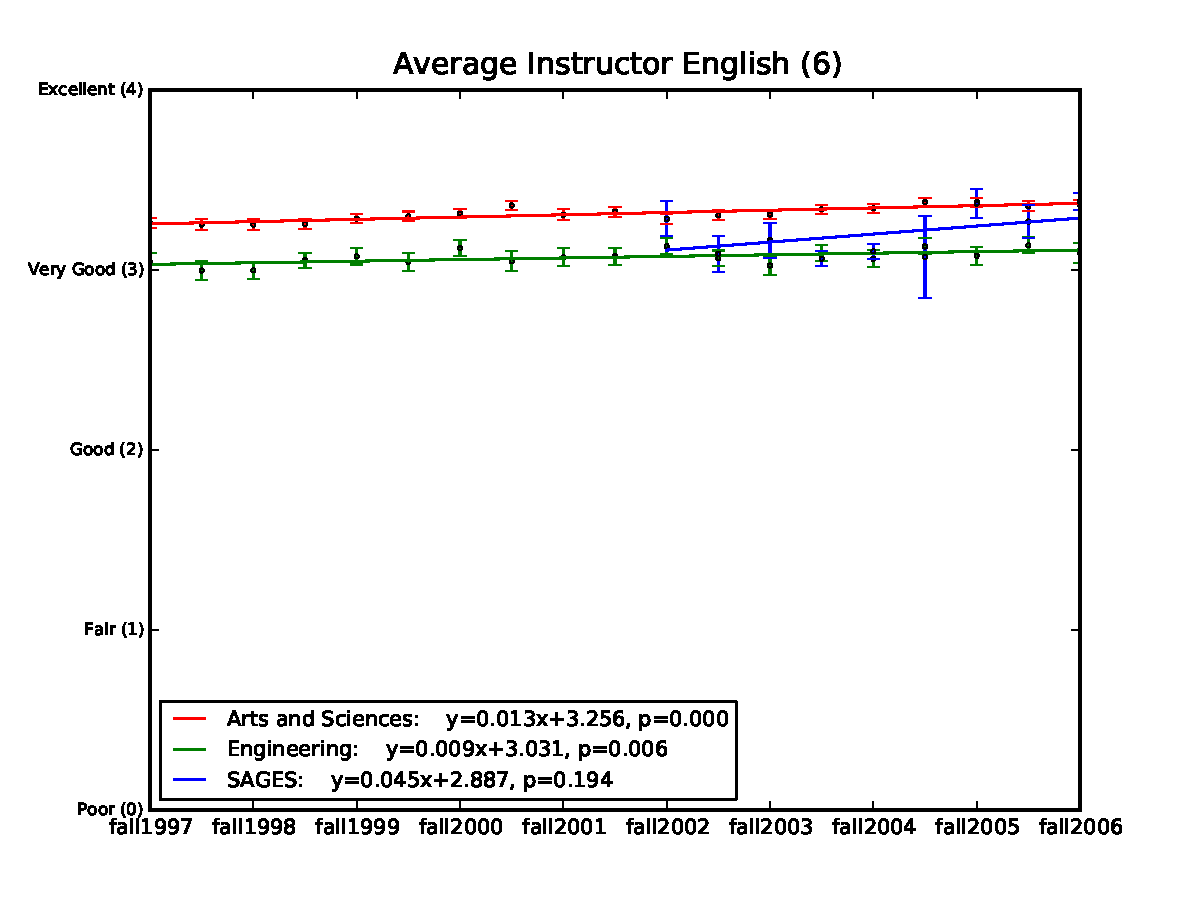
\includegraphics[width=5in]{figures/6_english_over_time.pdf} \\
    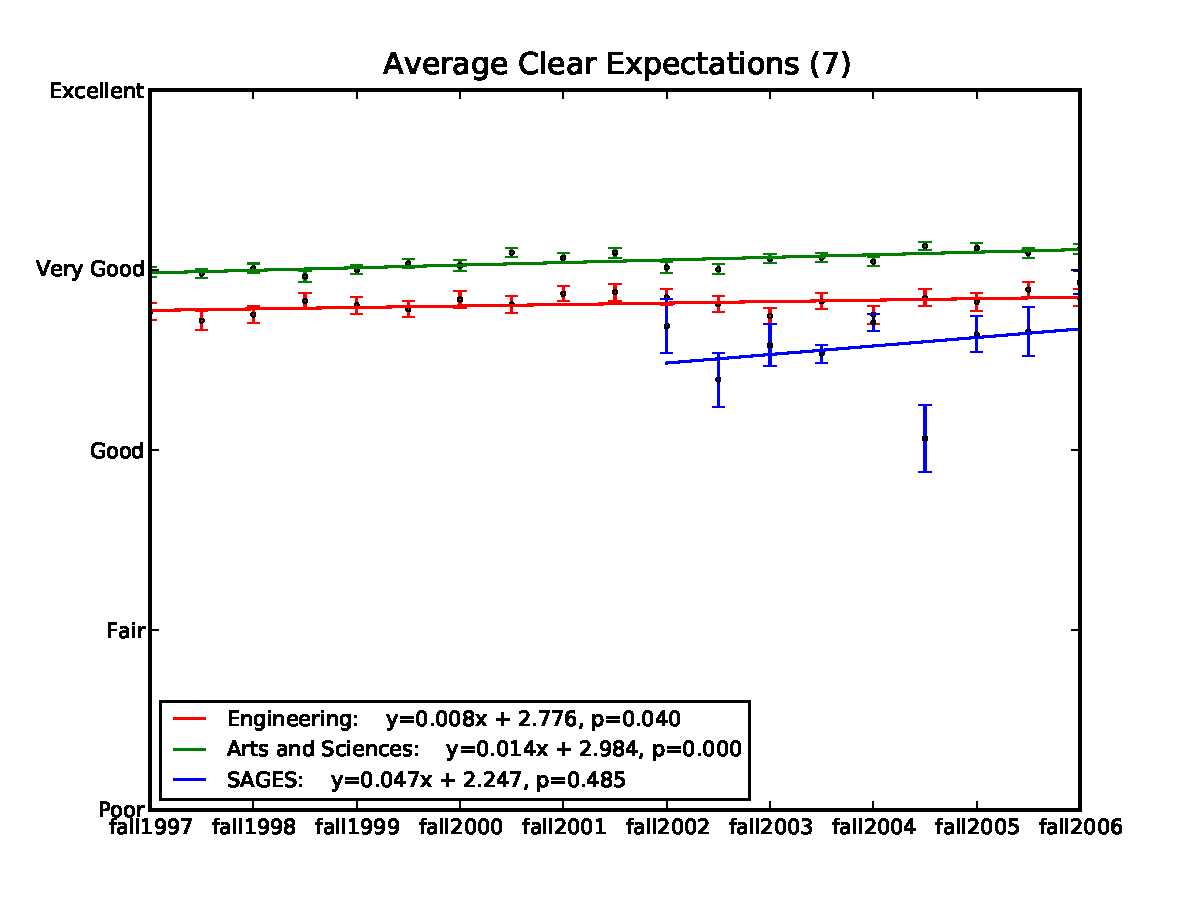
\includegraphics[width=5in]{figures/7_expectations_over_time.pdf} \\
    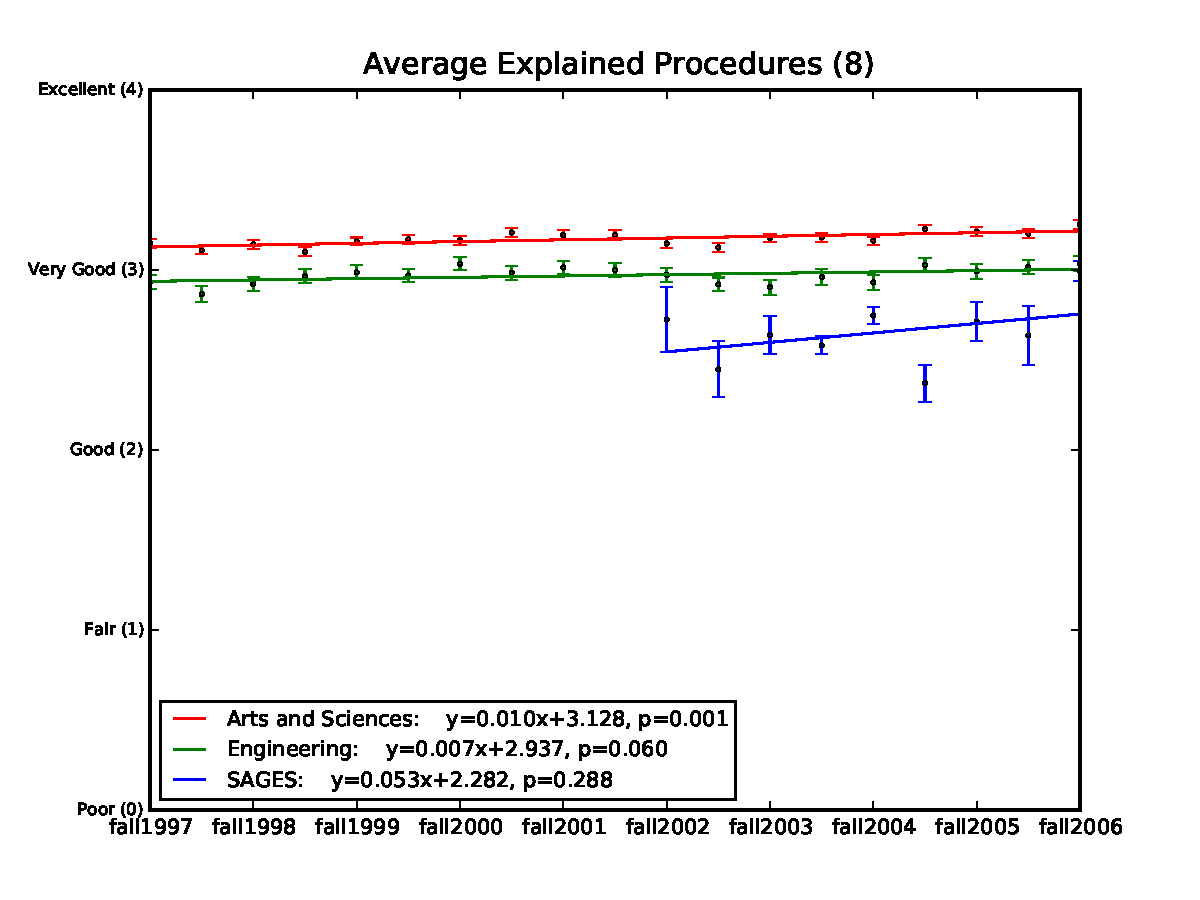
\includegraphics[width=5in]{figures/8_procedures_over_time.pdf} \\
    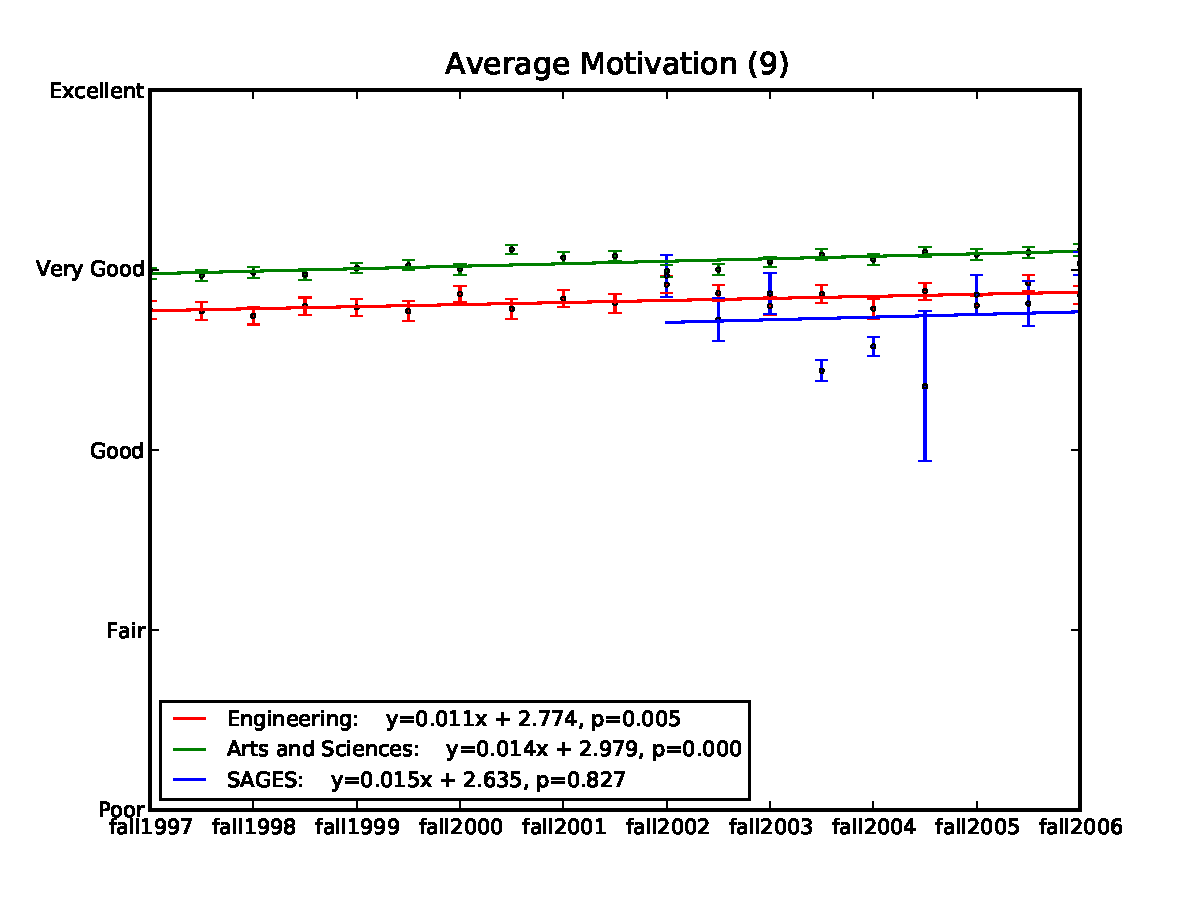
\includegraphics[width=5in]{figures/9_motivation_over_time.pdf} \\
    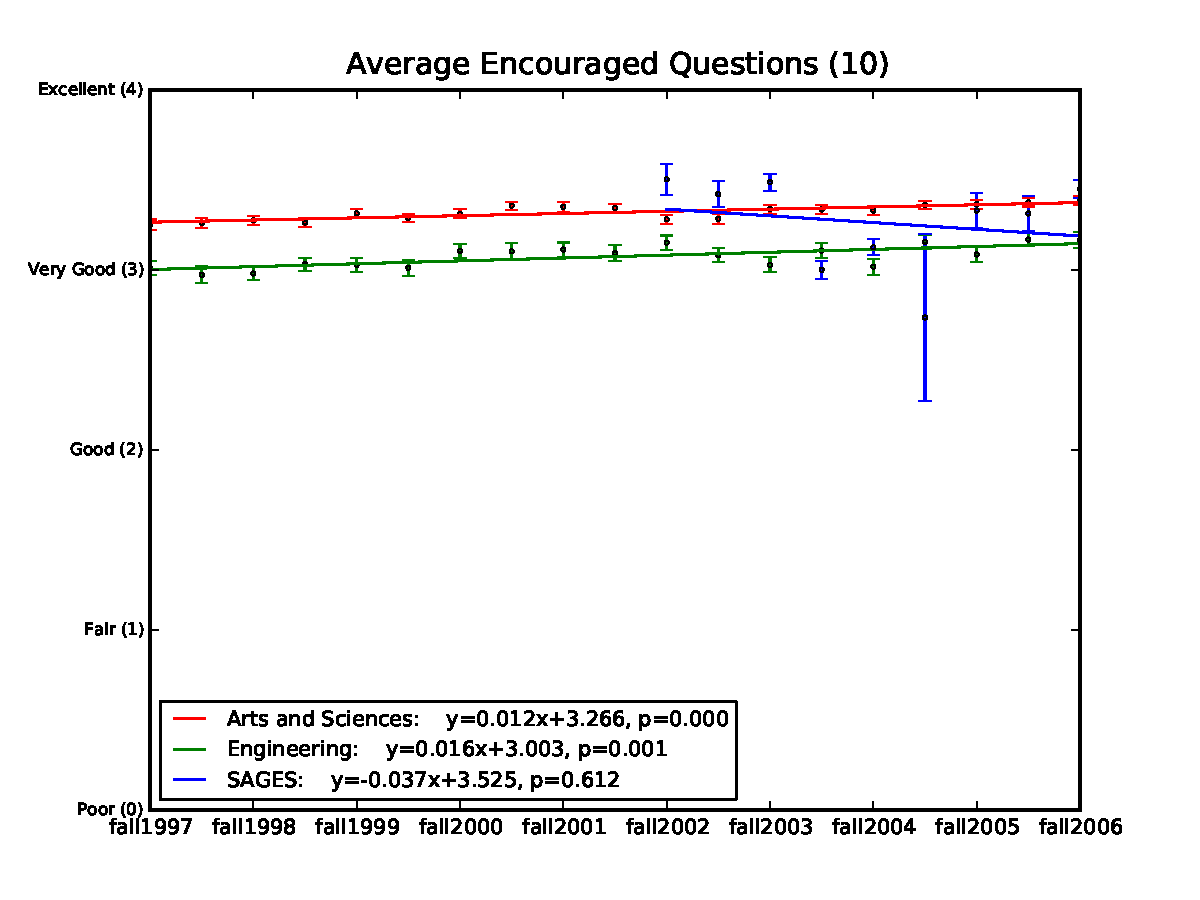
\includegraphics[width=5in]{figures/10_questions_over_time.pdf} \\
    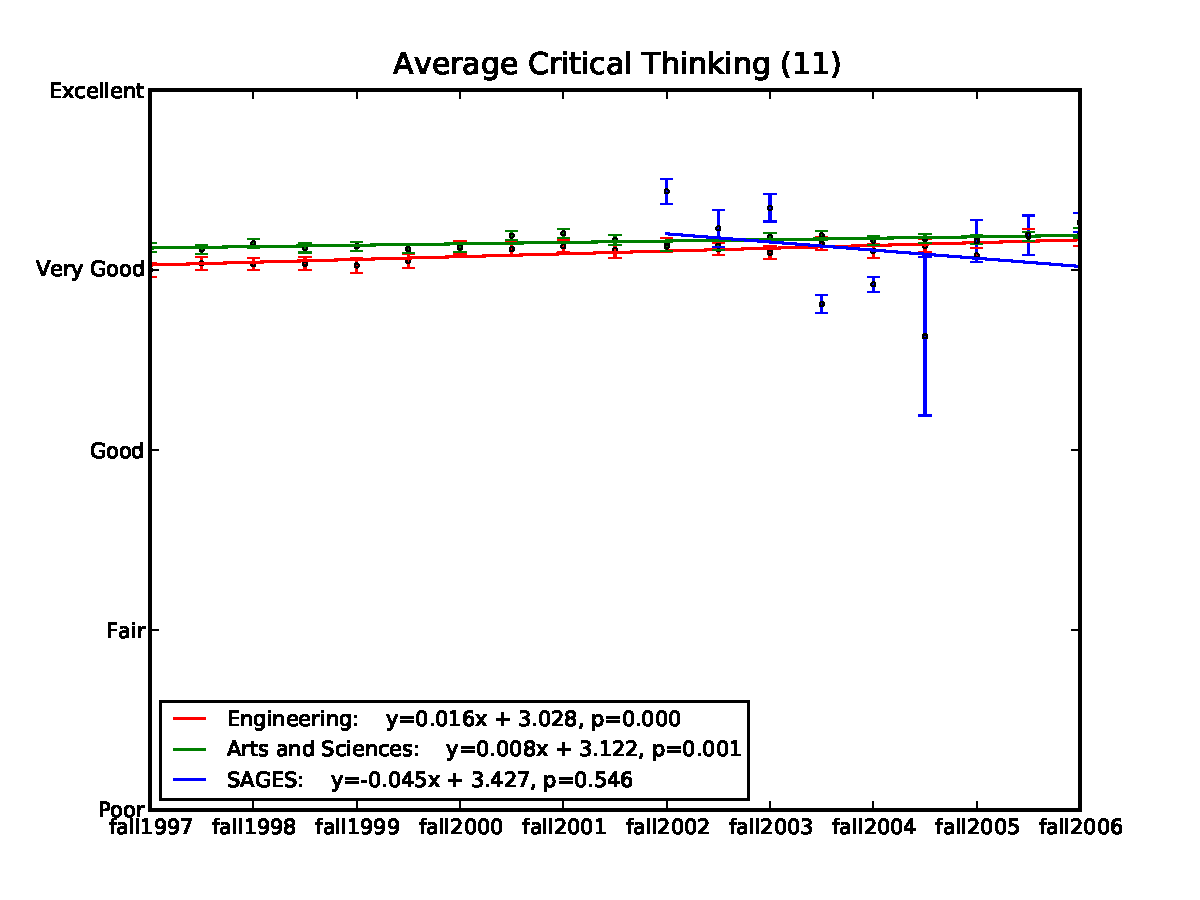
\includegraphics[width=5in]{figures/11_critthink_over_time.pdf} \\
    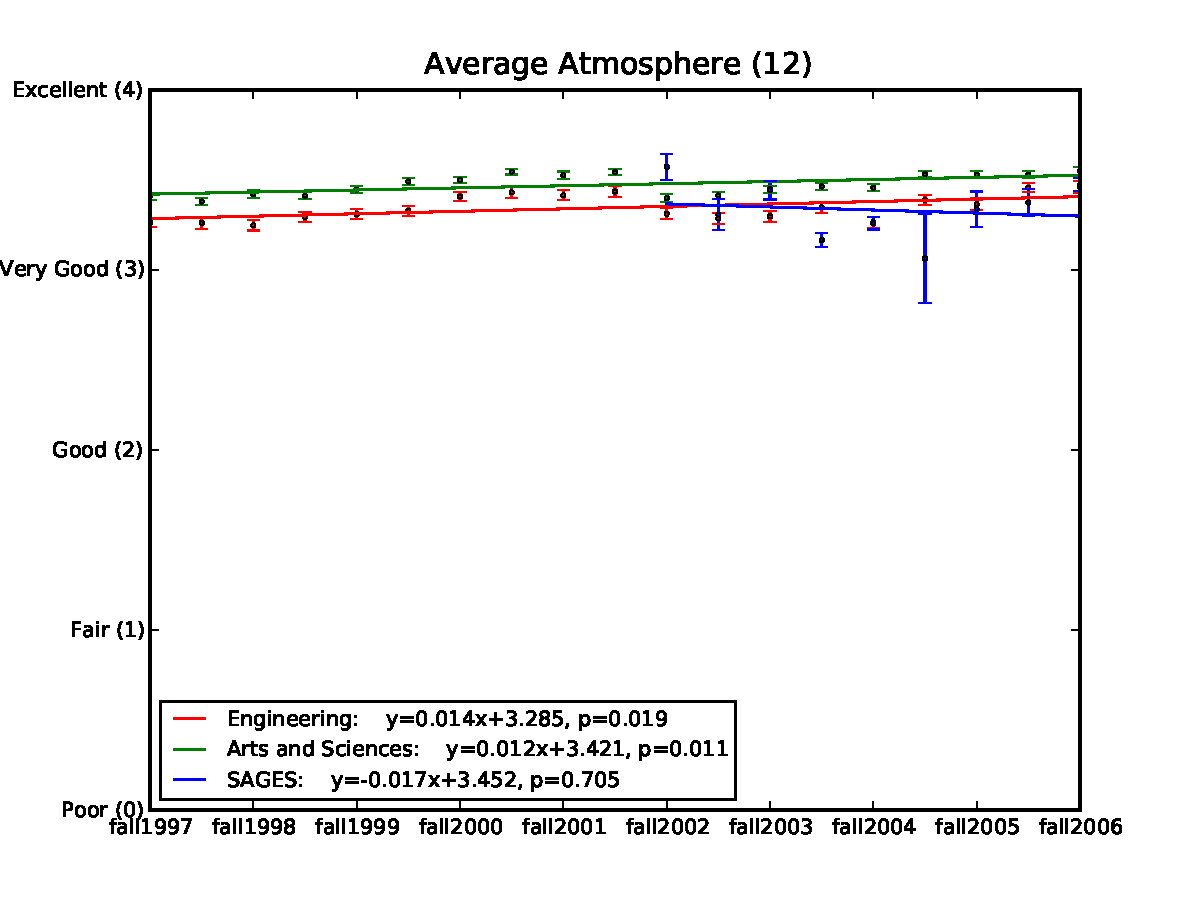
\includegraphics[width=5in]{figures/12_atmosphere_over_time.pdf} \\
    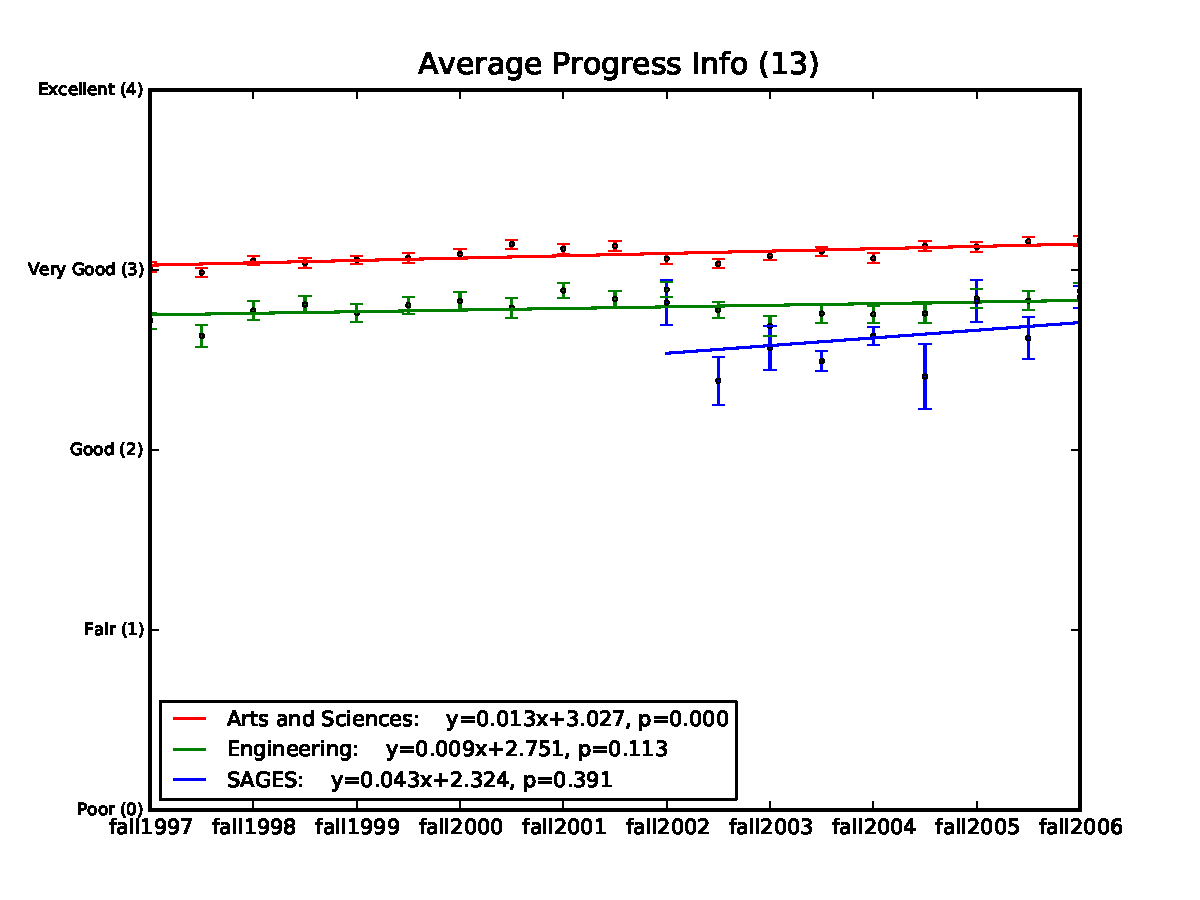
\includegraphics[width=5in]{figures/13_prog_info_over_time.pdf} \\
    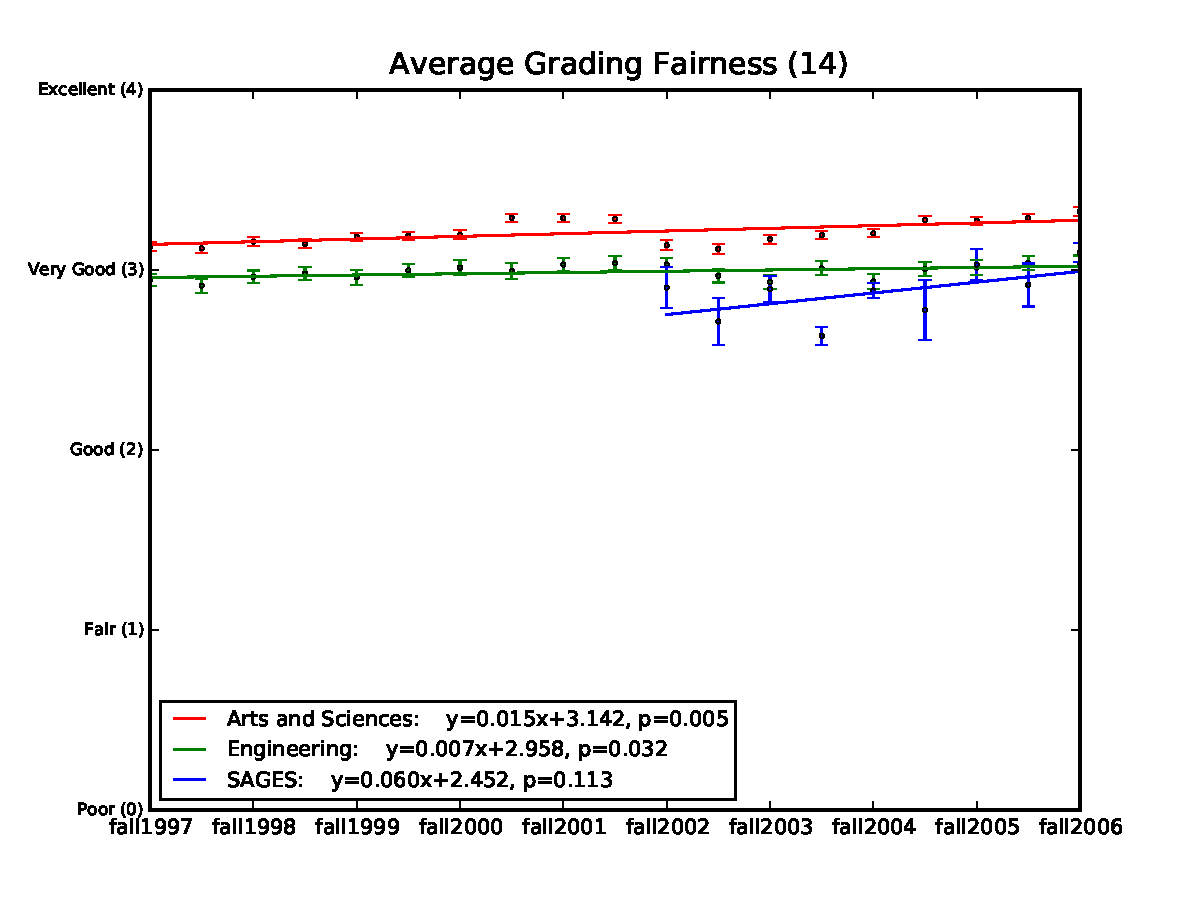
\includegraphics[width=5in]{figures/14_fair_grading_over_time.pdf} \\
    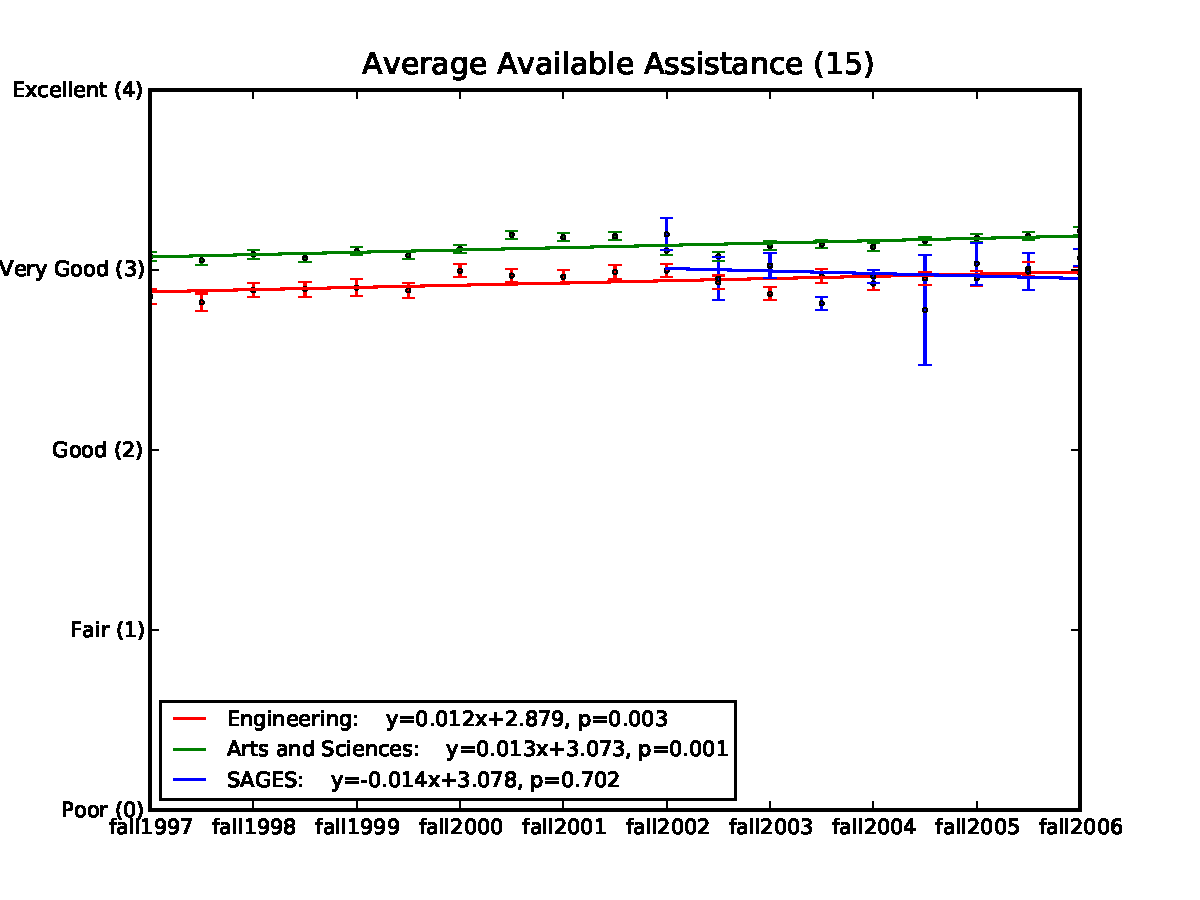
\includegraphics[width=5in]{figures/15_assistance_over_time.pdf} \\
    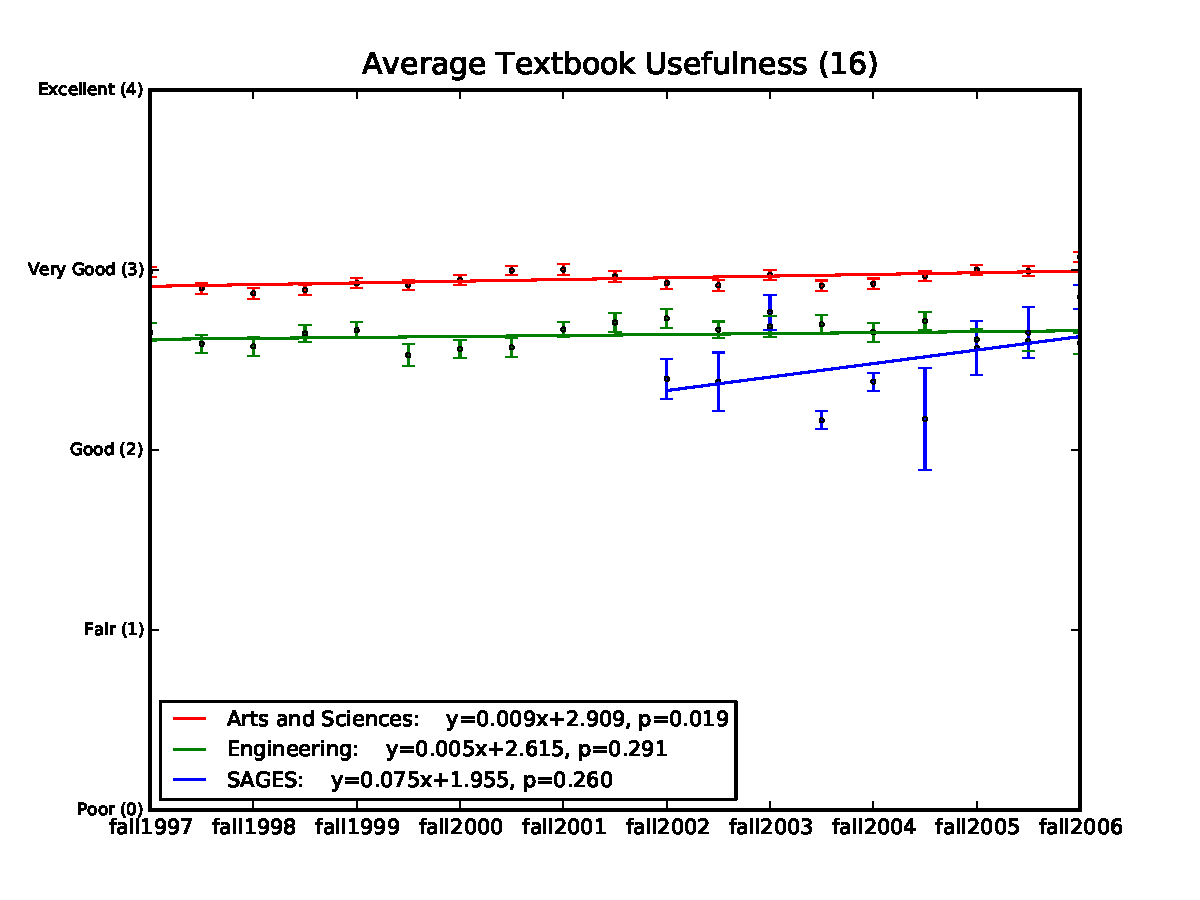
\includegraphics[width=5in]{figures/16_textbook_over_time.pdf} \\
    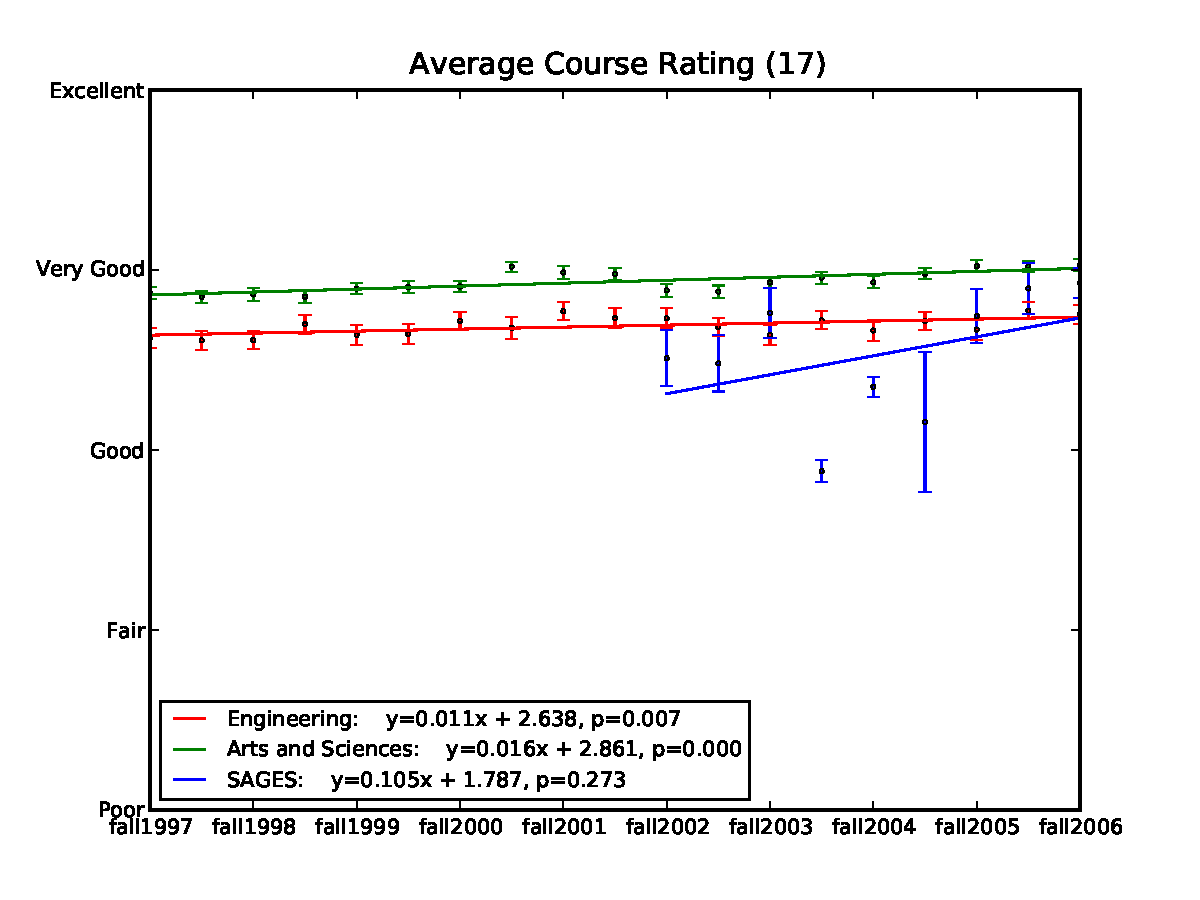
\includegraphics[width=5in]{figures/17_rating_over_time.pdf} \\
    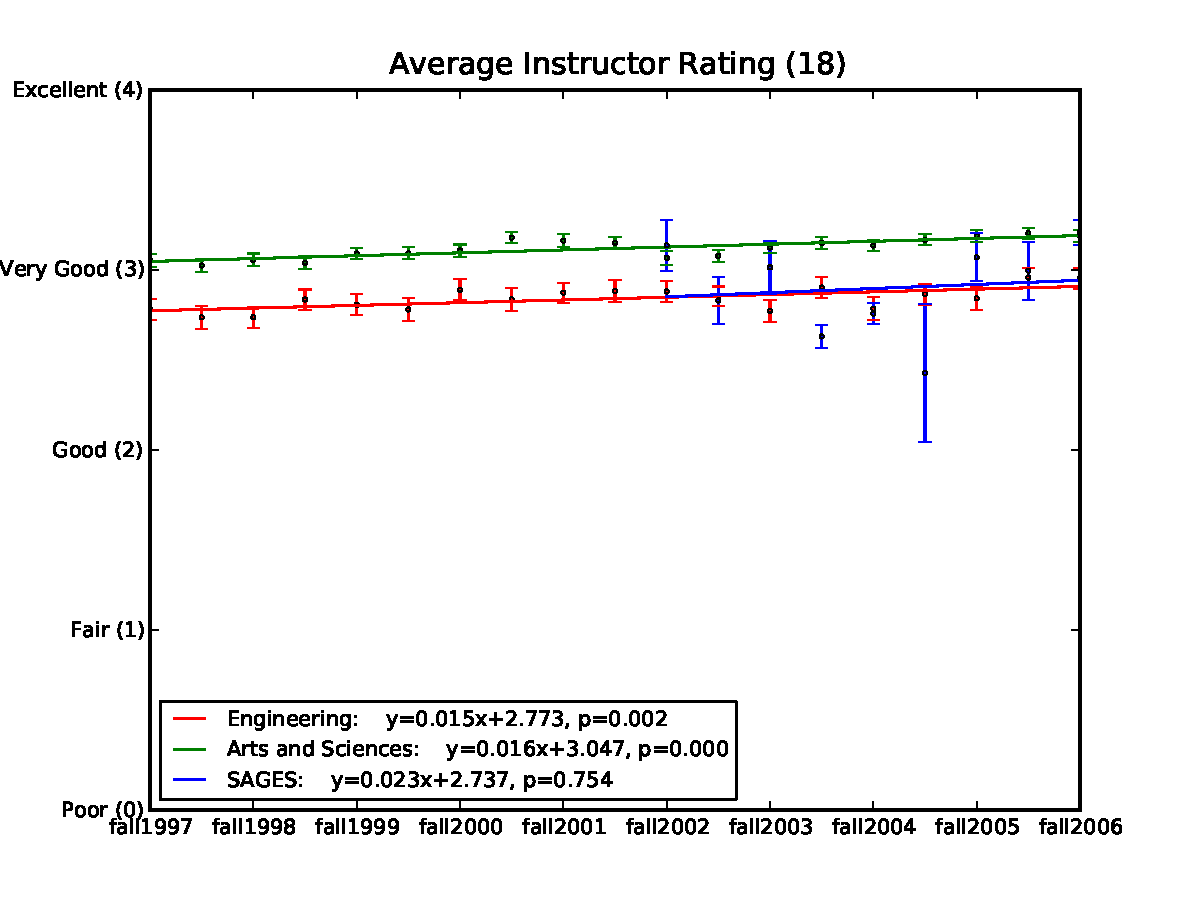
\includegraphics[width=5in]{figures/18_instructor_over_time.pdf} \\
    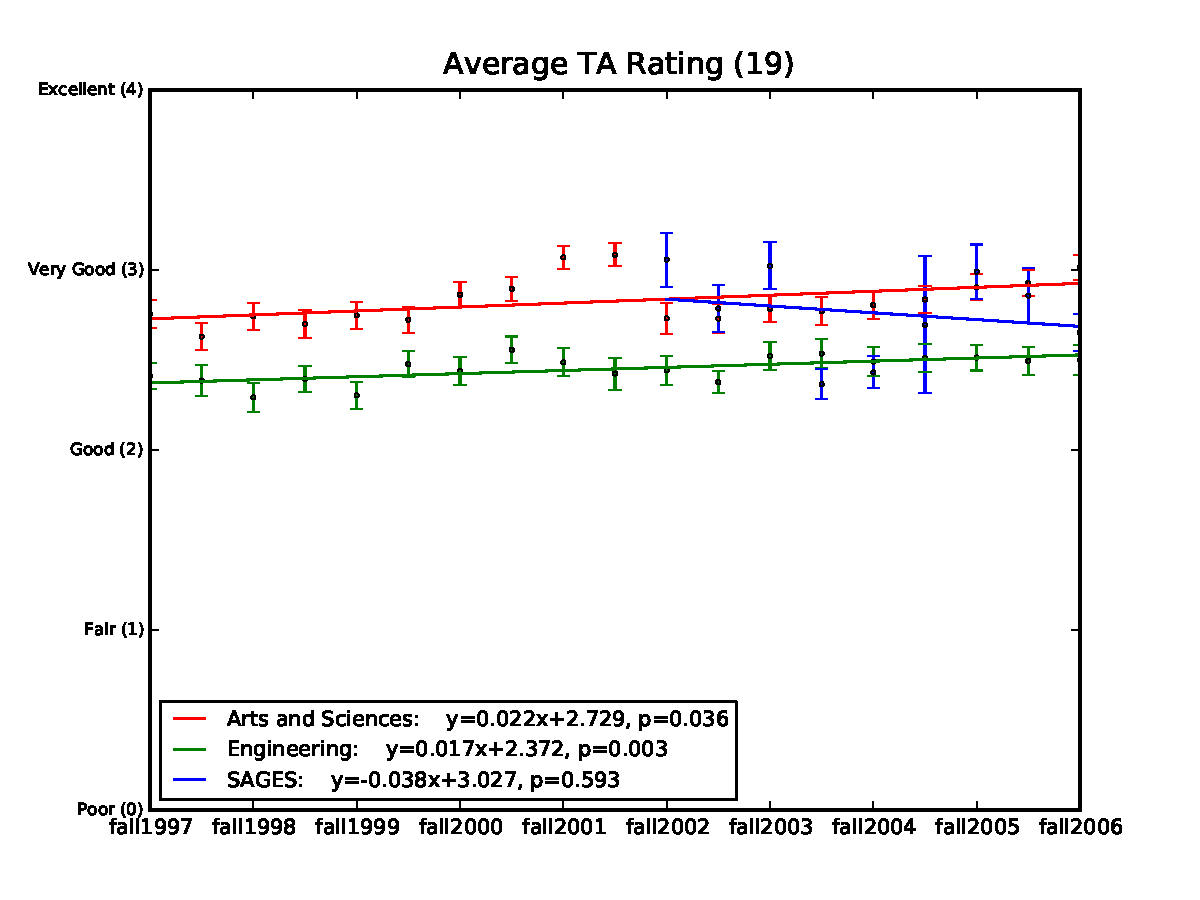
\includegraphics[width=5in]{figures/19_ta_over_time.pdf} \\
    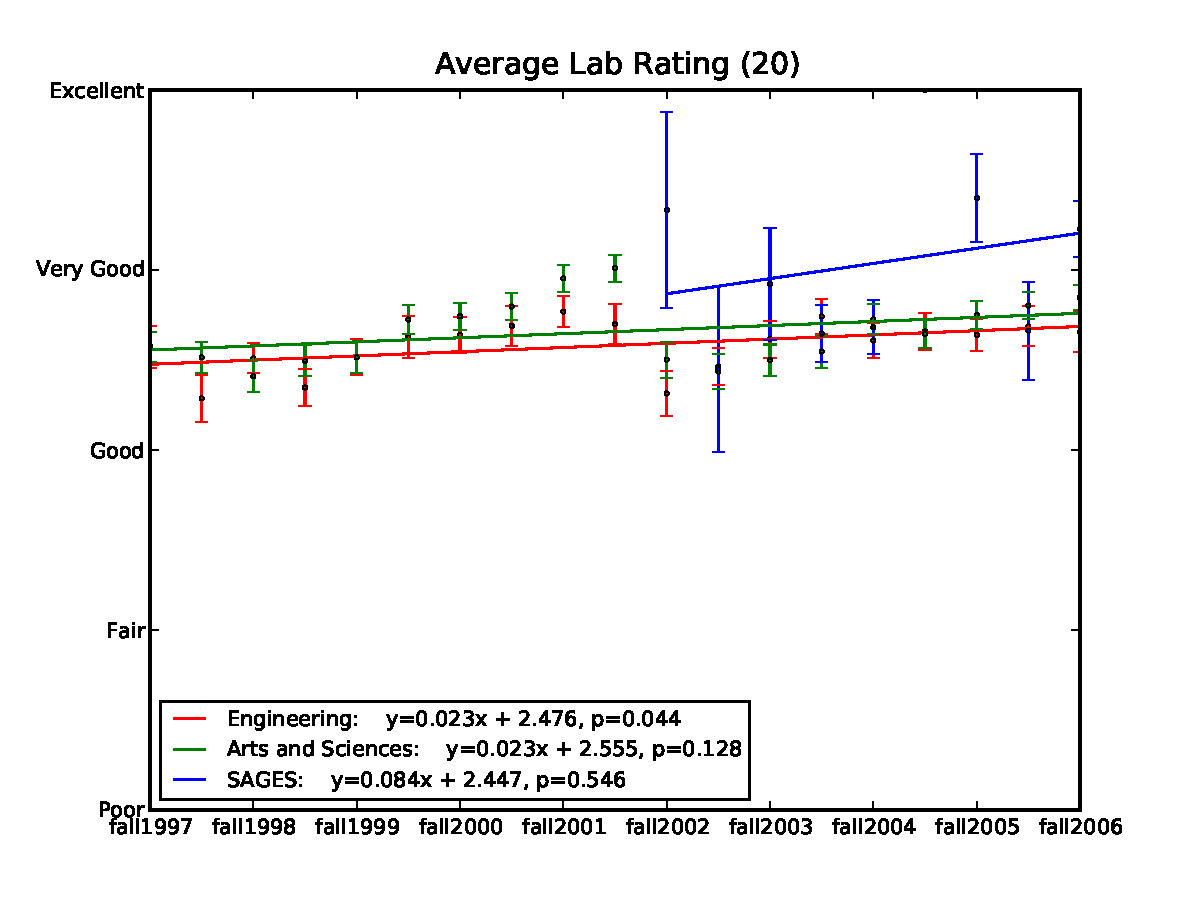
\includegraphics[width=5in]{figures/20_lab_over_time.pdf}
\end{center}


\end{document}
